%!TEX program = xelatex
\documentclass{article}
\usepackage{LaTeX-Submodule/template}

% Additional packages & macros

% Header and footer
\newcommand{\className}{Linear Algebra}
\newcommand{\classTime}{Semester 1, 2021}
\newcommand{\classInstructorName}{Dr Ravindra Pethiyagoda}

\fancyhf{}
\fancyhead[L]{\className}
\fancyhead[R]{\leftmark}
\fancyfoot[C]{\thepage}

% Copyright
\usepackage[
    type={CC},
    modifier={by-nc-sa},
    version={4.0},
    imagewidth={5em},
    hyphenation={raggedright}
]{doclicense}

\date{}

\begin{document}
%
\begin{titlepage}
    \vspace*{\fill}
    \begin{center}
        \LARGE{\textbf{\className}}
        \texorpdfstring{\\}{ }
        \texorpdfstring{\vspace{0.1in}}{ }
        \normalsize{\classTime}
        \texorpdfstring{\\}{ }
        \texorpdfstring{\vspace{0.1in}}{ }
        \normalsize\textit{\classInstructorName}
        \texorpdfstring{\\}{ }
        \texorpdfstring{\vspace{0.2in}}{ }
        \textsc{Tarang Janawalkar}
    \end{center}
    \vspace*{\fill}
    \doclicenseThis
    \thispagestyle{empty}
\end{titlepage}
\newpage
%
\tableofcontents 
\newpage
%
\section{Euclidean Vector Spaces}
	\subsection{Vectors}
	\begin{definition}
		An $n$-dimensional \textbf{vector} is an ordered list of $n$ numbers.
		\begin{equation*}
			\symbfit{v} = \mqty[v_1 \\ v_2 \\ \vdots \\ v_n] \in \mathbb{R}^n
		\end{equation*}
	\end{definition}
	\begin{theorem}
		$\mathbb{R}^n$ is the set of all ordered $n$-tuples of real numbers.
		\begin{equation*}
			\mathbb{R}^n = \bigl\{\left(v_1,\: v_2,\: \ldots,\: v_n\right): v_1,\: v_2,\: \ldots,\: v_n \in \mathbb{R}: n \in \mathbb{N}\bigr\}
		\end{equation*}
	\end{theorem}
	\underline{Notation:}

	\begin{enumerate}
		\item Component form: $\symbfit{v} = \left\langle{v_1,\: v_2}\right\rangle = \left(v_1,\: v_2\right) = \mqty(v_1 \\ v_2) = \mqty[v_1 \\ v_2]$
		\item Unit vector form: $\symbfit{v} = v_1\symbfit{\hat{i}} + v_2\symbfit{\hat{j}}$, where $\symbfit{\hat{i}}$ and $\symbfit{\hat{j}}$ are basis vectors along the $x$ and $y$ axes respectively.
		\item Denotation: $\symbfit{v} = \underset{\sim}{v} = \vec{v}$
	\end{enumerate}
	\subsection{Position and Displacement Vectors}
	\begin{definition}
		The \textbf{displacement vector} $\overrightarrow{AB}$ from $\symbfit{a}$ to $\symbfit{b}$ can be defined as $\symbfit{b}-\symbfit{a}$.
		\begin{figure}[H]
			\centering
			\includegraphics*{vector_position.pdf}
			\caption{Displacement vector between two points.}
		\end{figure}
	\end{definition}
	\subsection{Vector Addition}
		\begin{definition}
			\textbf{Vector addition} is performed by adding the corresponding components of two vectors of the same dimension.
			\begin{equation*}
				\symbfit{a} + \symbfit{b} =
				\mqty[
					a_1+b_1 \\
					\vdots \\
					a_n+b_n
				]
			\end{equation*}
		\end{definition}
	\subsection{Scalar Multiplication}
		\begin{definition}
			\textbf{Scalar multiplication} is performed by multiplying each element of the vector by the scalar. 
			\begin{equation*}
				a\symbfit{v} =
				\mqty[
					av_1 \\
					\vdots \\
					av_n
				]
			\end{equation*}
		\end{definition}
	\subsection{Norm of a Vector}
		\begin{definition}
			The \textbf{norm} of a vector $\symbfit{v}$, denoted by $\norm{\symbfit{v}}$, is the \textit{length} or \textit{magnitude} of $\symbfit{v}$.
			\begin{equation*}
				\norm{\symbfit{v}} = \sqrt{v_1^2 + v_2^2+\cdots+v_n^2}
			\end{equation*}
		\end{definition}
	\subsection{The Unit Vector}
		\begin{definition}
			A \textbf{unit vector} is a vector, denoted $\symbfit{\hat{v}}$, that has a length of 1 in the direction of $\symbfit{v}$.
			\begin{equation*}
				\symbfit{\hat{v}} = \frac{\symbfit{v}}{\norm{\symbfit{v}}}
			\end{equation*}
		\end{definition}
	\subsection{The Dot Product}
		\begin{definition}
			The \textbf{dot product} is a function that associates each pair of vectors $\symbfit{v},\: \symbfit{w} \in \mathbb{R}^n$ a real number $\symbfit{v}\cdot\symbfit{w}$.
			\begin{align*}
				\symbfit{v}\cdot\symbfit{w} &= v_1 w_1 + v_2 w_2 + \cdots + v_n w_n \\
									&= \norm{\symbfit{v}} \norm{\symbfit{w}} \cos{\left(\theta\right)}
			\end{align*}
			where $\theta$ is the angle between $\symbfit{v}$ and $\symbfit{w}$.
		\end{definition}
		\begin{theorem}
			If $\symbfit{v} \cdot \symbfit{w}=0$ then $\symbfit{v}$ and $\symbfit{w}$ are orthogonal. 
		\end{theorem} 
	\subsection{The Cross Product}
		\begin{definition}
			The \textbf{cross product} is a function that associates each ordered pair of vectors $\symbfit{v},\: \symbfit{w}\in \mathbb{R}^3$ a vector $\symbfit{v}\times\symbfit{w}\in \mathbb{R}^3$.
			\begin{align*}
				\symbfit{v}\times\symbfit{w} &= 
				\mqty|
					\symbfit{\hat{i}} & \symbfit{\hat{j}} & \symbfit{\hat{k}} \\
					v_1 & v_2 & v_3 \\
					w_1 & w_2 & w_3
				| \\
				&= \norm{\symbfit{v}}\norm{\symbfit{w}}\sin{\left(\theta\right)}\symbfit{\hat{n}}
			\end{align*}
			where $\symbfit{\hat{n}}$ is the normal vector given by the right-hand rule.
		\end{definition}
	\newpage
\section{Vector Identities}
	\begin{theorem}
		Commutativity of vector addition.
		\begin{equation*}
			\symbfit{a} + \symbfit{b} = \symbfit{b} + \symbfit{a}
		\end{equation*}
	\end{theorem}
	\begin{theorem}
		\begin{equation*}
			\symbfit{a}\cdot\symbfit{a}=\norm{\symbfit{a}}^2
		\end{equation*}
	\end{theorem}
	\begin{theorem}
		Commutativity of dot products.
		\begin{equation*}
			\symbfit{a}\cdot \symbfit{b} = \symbfit{b}\cdot \symbfit{a}
		\end{equation*}
	\end{theorem}
	\begin{theorem}
		Distributivity of dot products over vector addition.
		\begin{equation*}
			\symbfit{a}\cdot \left(\symbfit{b}+\symbfit{c}\right) = \symbfit{a}\cdot\symbfit{b} + \symbfit{a}\cdot\symbfit{c}
		\end{equation*}
	\end{theorem}
	\begin{theorem}
		Associativity of dot products over scalar multiplication.
		\begin{equation*}
			\left(r\symbfit{a}\right)\cdot\symbfit{b} = r\left(\symbfit{a}\cdot\symbfit{b}\right)=\symbfit{a}\cdot\left(r\symbfit{b}\right)
		\end{equation*}
	\end{theorem}
	\begin{theorem}
		Bilinearity of dot products.
		\begin{equation*}
			\symbfit{a}\cdot\left(r\symbfit{b}+\symbfit{c}\right)=r\left(\symbfit{a}\cdot\symbfit{b}\right)+\left(\symbfit{a}\cdot\symbfit{c}\right)
		\end{equation*}
	\end{theorem}
	\begin{theorem}
		\begin{equation*}
			\symbfit{a}\times \symbfit{a} = \symbfup{0}
		\end{equation*}
	\end{theorem}
	\begin{theorem}
		Anticommutativity of cross products.
		\begin{equation*}
			\symbfit{a}\times \symbfit{b} = -\symbfit{b}\times \symbfit{a}
		\end{equation*}
	\end{theorem}
	\begin{theorem}
		Distributivity of cross products over vector addition.
		\begin{equation*}
			\symbfit{a}\times\left( \symbfit{b}+\symbfit{c} \right) = \symbfit{a}\times\symbfit{b} + \symbfit{a}\times\symbfit{c}
		\end{equation*}
	\end{theorem}
	\begin{theorem}
		Associativity of cross products over scalar multiplication.
		\begin{equation*}
			\left( r \symbfit{a}\right)\times\symbfit{b} = \symbfit{a}\times\left( r \symbfit{b} \right) = r\left(\symbfit{a}\times\symbfit{b}\right)
		\end{equation*}
	\end{theorem}
	\begin{theorem}
		\begin{equation*}
			\symbfit{a} \cdot \left(\symbfit{b}\times\symbfit{c}\right) = \symbfit{b} \cdot \left(\symbfit{c}\times\symbfit{a}\right) = \symbfit{c} \cdot \left(\symbfit{a}\times\symbfit{b}\right)
		\end{equation*}
	\end{theorem}
	\begin{theorem}
		\begin{equation*}
			\symbfit{a} \times \left(\symbfit{b}\times\symbfit{c}\right) = \symbfit{b} \left(\symbfit{a}\cdot\symbfit{c}\right) - \symbfit{c}\left(\symbfit{a}\cdot\symbfit{b}\right)
		\end{equation*}
	\end{theorem}
	\newpage
\section{Linear System of Equations}
	\subsection{Linear Equations}
	\begin{definition}
		A \textbf{linear equation} in $n$ variables $x_1,\: x_2,\: \dots, x_n$ can be expressed in the form
		\begin{equation*}
			a_{1}x_1 + a_{2}x_2 + \dots + a_{n}x_n = b
		\end{equation*}
		where the \textit{coefficients} $a_1,\: a_2,\: \dots, a_n$ and the \textit{constant term} $b$ are constants.
	\end{definition}
	\subsection{Homogeneous Linear Equations}
	\begin{definition}
		In the special case where $b=0$, the linear equation is called a \textbf{homogeneous linear equation}.
	\end{definition}
	\subsection{Linear Systems}
	\begin{definition}
		A \textbf{linear system of equations} is a set of linear equations, where the variables $x_i$ are called \textit{unknowns}. The general linear system of $m$ equations with $n$ unknowns can be written as
		\begin{equation*}
			\left\{
			\setlength\arraycolsep{0pt}
			\begin{array}{ c >{{}}c<{{}} c >{{}}c<{{}} c >{{}}c<{{}} c >{{}}c<{{}} c }
			a_{11}x_1                         &+& a_{12}x_2                         &+& \cdots &+& a_{1n}x_n                         &=& b_1 \\
			a_{21}x_1                         &+& a_{22}x_2                         &+& \cdots &+& a_{2n}x_n                         &=& b_2 \\
			\vdotswithin{a_{31}}\phantom{x_1} & & \vdotswithin{a_{32}}\phantom{x_2} & &        & & \vdotswithin{a_{3n}}\phantom{x_n} & & \vdots \\ 
			a_{m1}x_1                         &+& a_{m2}x_2                         &+& \cdots &+& a_{mn}x_n                         &=& b_m
			\end{array}
			\right.
		\end{equation*}
		A \textbf{solution} to the system is an $n$-tuple $\left\langle x_1,\: x_2,\:\dots,\:x_n\right\rangle$ that satisfies each equation.
	\end{definition}
	\subsection{Coefficient Matrices}
	\begin{definition}
		The coefficients of the variables in each equation can be placed inside the systems \textbf{coefficient matrix}.
		\begin{equation*}
			\mqty[
				a_{11} & a_{12} & \cdots & a_{1n} \\
				a_{21} & a_{22} & \cdots & a_{2n} \\
				\vdots & \vdots &        & \vdots \\
				a_{m1} & a_{m2} & \cdots & a_{mn}
			]
		\end{equation*}
	\end{definition}
	\subsection{Augmented Matrices}
	\begin{definition}
		The information of a system can be contained in its \textbf{augmented matrix}.
		\begin{equation*}
			\left[\begin{array}{cccc|c}
				a_{11} & a_{12} & \cdots & a_{1n} & b_1 \\
				a_{21} & a_{22} & \cdots & a_{2n} & b_2 \\
				\vdots & \vdots &        & \vdots & \vdots \\
				a_{m1} & a_{m2} & \cdots & a_{mn} & b_m
			\end{array}\right]
		\end{equation*}
	\end{definition}
	\begin{definition}
		An array having $m$ rows and $n$ columns, is an $m \times n$ \textbf{matrix}. This matrix may be denoted as $a_{ij}$, where $a_{ij}$ is the entry in $i$th row and $j$th column of the matrix $\symbfit{A}$.
		\begin{equation*}
			\text{$m$ rows} 
			\left\{
				\left[
					\vphantom{\begin{array}{c} 1 \\ 1 \\ 1 \\ 1 \end{array}}
					\smash{\underbrace{
						\begin{array}{cccc}
							a_{11} & a_{12} & \cdots & a_{1n} \\
							a_{21} & a_{22} & \cdots & a_{2n} \\
							\vdots & \vdots &        & \vdots \\
							a_{m1} & a_{m2} & \cdots & a_{mn}
						\end{array}
					}_{\text{$n$ columns}}}
				\right]
			\right.
		\end{equation*}
	\end{definition}
	\subsection{Elementary Row Operations}
	\begin{definition}
		A linear system can be solved using the following \textbf{elementary row operations}:
		\begin{enumerate}
			\item \textbf{scalar multiplication}: multiplying any row by a constant
			\item \textbf{row addition}: adding a multiple of one row to another
			\item \textbf{row exchange}: exchanging any two rows
		\end{enumerate}
	\subsection{Pivots}
	\end{definition}
	\begin{definition}
		The first non-zero entry of the row in a matrix is called the \textbf{pivot} of the row.
	\end{definition}
	\begin{theorem} \label{theorem:pivots}
		If a row apart from the first has a pivot, then this pivot must be to the \textit{right} of the pivot in the preceding row.
	\end{theorem}
	\subsection{Gaussian Elimination}
	\begin{definition}
		\textbf{Gaussian elimination} is a method for solving linear systems. These systems can be solved by composing the augmented matrix of a system, and performing elementary row operations, to put the matrix in the form
		\begin{equation*}
			\mqty[
				a_{11} & a_{12} & \cdots & a_{1n} \\
				  	   & a_{22} & \cdots & a_{2n} \\
				  	   &        & \ddots & \vdots \\
				  	   &        &        & a_{mn}]
		\end{equation*}
	\end{definition}
	\subsection{Row-Echelon Form}
	\begin{definition}
		A matrix that has undergone Gaussian elimination is in \textbf{row-echelon form} if the pivots of the augmented matrix are all 1.
		\begin{equation*}
			\mqty[
				1 & a_{12} & \cdots & a_{1n} \\
				  & 1      & \cdots & a_{2n} \\
				  &        & \ddots & \vdots \\
				  &        &        & 1]
		\end{equation*}
	\end{definition}
	\subsection{Gauss-Jordan Elimination}
	\begin{definition}
		\textbf{Gauss-Jordan elimination} extends Gaussian elimination so that the entries in a column containing a pivot are zeros, and the pivots are all 1. This new augmented matrix is then in \textbf{reduced row-echelon form}. matrix is in \textbf{reduced row-echelon form}.
		\begin{equation*}
			\mqty[
				1 &   &        & \\
				  & 1 &        & \\
				  &   & \ddots & \\
				  &   &        & 1]
		\end{equation*}
	\end{definition}
	\subsection{Solutions to Linear Systems}
	\begin{definition}
		A \textbf{consistent system} of equations has at least one solution, and an \linebreak \textbf{inconsistent system} has no solution. 
	\end{definition}
	\newpage
\section{Matrices}
	\begin{definition}
		A \textbf{matrix} is an array of numbers arranged into \textit{rows} and \textit{columns}, and can be used to represent a linear transformation.
		\begin{equation*}
			\symbfit{A} = \mqty[
				a_{11} & a_{12} & \cdots & a_{1n} \\
				a_{21} & a_{22} & \cdots & a_{2n} \\
				\vdots & \vdots &        & \vdots \\
				a_{m1} & a_{m2} & \cdots & a_{mn} \\
				] \in \mathbb{R}^{m \times n}
		\end{equation*}
	\end{definition}
	\subsection{Matrix Addition}
	\begin{definition}
		\textbf{Matrix addition} is performed by adding the corresponding components of two matrices of the same dimension.
		\begin{equation*}
			\symbfit{A} + \symbfit{B} = \mqty[
				a_{11} + b_{11} & a_{12} + b_{12} & \cdots & a_{1n} + b_{1n} \\
				a_{21} + b_{21} & a_{22} + b_{22} & \cdots & a_{2n} + b_{2n} \\
				\vdots          & \vdots          &        & \vdots          \\
				a_{m1} + b_{m1} & a_{m2} + b_{m2} & \cdots & a_{mn} + b_{mn} \\
				]
		\end{equation*}
	\end{definition}
	\subsection{Scalar Multiplication}
	\begin{definition}
		\textbf{Scalar multiplication} is performed by multiplying each element of a matrix by a scalar. 
		\begin{equation*}
			c\symbfit{A} = \mqty[
				ca_{11} & ca_{12} & \cdots & ca_{1n} \\
				ca_{21} & ca_{22} & \cdots & ca_{2n} \\
				\vdots  & \vdots  &        & \vdots  \\
				ca_{m1} & ca_{m2} & \cdots & ca_{mn} \\
				]
		\end{equation*}
	\end{definition}
	\subsection{Matrix Multiplication}	
	\begin{definition}
		\textbf{Matrix multiplication} is performed by multiplying each row in the first matrix by the columns of the second matrix.
 		\begin{align*}
			\symbfit{A} \symbfit{B} &= \symbfit{C} \\
			\mqty[
				\horzbar & \symbfit{a}_{1}  & \horzbar \\
				\horzbar & \symbfit{a}_{2}  & \horzbar \\
				         & \vdots           & \\
				\horzbar & \symbfit{a}_{m}  & \horzbar 
			]
			\mqty[
				\vertbar        & \vertbar        &         & \vertbar \\
				\symbfit{b}_{1} & \symbfit{b}_{2} & \cdots  & \symbfit{b}_{n} \\
				\vertbar        & \vertbar        &         & \vertbar
			] &=
			\mqty[
				\symbfit{a}_1\symbfit{b}_1 & \symbfit{a}_1\symbfit{b}_2 & \cdots & \symbfit{a}_1\symbfit{b}_n \\
				\symbfit{a}_2\symbfit{b}_1 & \symbfit{a}_2\symbfit{b}_2 & \cdots & \symbfit{a}_2\symbfit{b}_n \\
				\vdots                     & \vdots                     &        & \vdots \\
				\symbfit{a}_m\symbfit{b}_1 & \symbfit{a}_m\symbfit{b}_2 & \cdots & \symbfit{a}_m\symbfit{b}_n
			]
		\end{align*}
	\end{definition}
	\begin{theorem}
		A matrix product is defined if and only if the number of columns in the first matrix is equal to the number of rows in the second matrix.
	\end{theorem}
	\subsection{The Identity Matrix}
	\begin{definition}
		The \textbf{identity matrix} is the simplest nontrivial \textbf{diagonal matrix}, denoted $\mathbb{1}$, such that
		\begin{equation*}
			\mathbb{1} \symbfit{A} = \symbfit{A} 
		\end{equation*}
		written explicitly as
		\begin{equation*}
			\mathbb{1} = \mqty[
				1 &   &        & \\
			      & 1 &        & \\
				  &   & \ddots & \\
				  &   &        & 1
			]
		\end{equation*}
	\end{definition}
	\subsection{The Inverse Matrix}
	\begin{definition}
		The \textbf{inverse} of a \textbf{square matrix} is a matrix $\symbfit{A}^{-1}$, such that
		\begin{equation*}
			\symbfit{A} \symbfit{A}^{-1} = \mathbb{1}
		\end{equation*}
	\end{definition}
	\begin{theorem}
		The inverse of a $2\times 2$ matrix is given by
		\begin{equation*}
			\symbfit{A}^{-1} = \frac{1}{ad-bc}
			\mqty[
				a_{22}  & -a_{12} \\
				-a_{21} & a_{11}
			]
		\end{equation*}
	\end{theorem}
	\begin{theorem}
		The inverse of an $n\times n$ matrix can be determined by solving $\left[\begin{array}{c|c} \symbfit{A} & \mathbb{1} \end{array}\right]$.
	\end{theorem}
	\subsection{The Diagonal Matrix}
	\begin{definition}
		A \textbf{diagonal} matrix, denoted $\diag{\left( d_{11},\: d_{22},\: \ldots,\: d_{nn} \right)}$, is an $n \times n$ matrix $\symbfit{D}$ in which entries outside the main diagonal are all zero. 
		\begin{equation*}
			\symbfit{D} = \diag{\left( d_{11}, d_{22}, \ldots, d_{nn} \right)}
			=\mqty[
				d_{11} &        &        & \\
				       & d_{22} &        & \\
					   &        & \ddots & \\
					   &        &        & d_{nn}
			]
		\end{equation*}
	\end{definition}
	\subsection{Matrix Transpose}
	\begin{definition}
		The \textbf{transpose} of a matrix, denoted by $\symbfit{A}^\top$, is obtained by replacing all $a_{ij}$ elements with $a_{ji}$, so that the matrix $\symbfit{A}$ is flipped over its main diagonal.
	\end{definition}
	\subsection{Matrix Trace}
	\begin{definition}
		The \textbf{trace} of an $n \times n$ matrix $\symbfit{A}$, denoted $\tr{\left( \symbfit{A} \right)}$, is defined as
		\begin{equation*}
			\tr{\left( \symbfit{A} \right)} = \sum_{i=1}^n a_{ii}
		\end{equation*}
	\end{definition}
	\newpage
\section{General Vector Spaces}
	\subsection{Real Vector Spaces}
	\begin{definition}
		A \textbf{vector space} is a set that is closed under vector addition and scalar \linebreak multiplication.
	\end{definition}
	\begin{theorem}
		If the following axioms are satisfied by all objects $\symbfit{u},\: \symbfit{v},\: \symbfit{w} \in V$, and all scalars $k$ and $m$, then $V$ is a \textbf{vector space}, and the objects in $V$ are vectors.
	\end{theorem}
	\begin{axiom}[Closure under addition] 
		\begin{equation*} \label{axiom:5_1_1}
			\symbfit{u}+\symbfit{v} \in V 
		\end{equation*}
	\end{axiom}
	\begin{axiom}[Commutativity of vector addition] 
		\begin{equation*} \label{axiom:5_1_2}
			\symbfit{u} + \symbfit{v} = \symbfit{v} + \symbfit{u}
		\end{equation*}
	\end{axiom}
	\begin{axiom}[Associativity of vector addition] 
		\begin{equation*} \label{axiom:5_1_3}
			\symbfit{u} + \left(\symbfit{v} + \symbfit{w}\right) = \left(\symbfit{u} + \symbfit{v}\right) + \symbfit{w}
		\end{equation*}
	\end{axiom}
	\begin{axiom}[Additive identity] 
		\begin{equation*} \label{axiom:5_1_4}
			\symbfit{u} + \symbfup{0} = \symbfit{u}
		\end{equation*}
	\end{axiom}
	\begin{axiom}[Additive inverse] 
		\begin{equation*} \label{axiom:5_1_5}
			\symbfit{u} + \left(-\symbfit{u}\right) = \symbfup{0}
		\end{equation*}
	\end{axiom}
	\begin{axiom}[Closure under scalar multiplication] 
		\begin{equation*} \label{axiom:5_1_6}
			k\symbfit{u} \in V
		\end{equation*}
	\end{axiom}
	\begin{axiom}[Distributivity of vector addition] 
		\begin{equation*} \label{axiom:5_1_7}
			k \left(\symbfit{u} + \symbfit{v}\right) = k\symbfit{u} + k\symbfit{v}
		\end{equation*}
	\end{axiom}
	\begin{axiom}[Distributivity of scalar addition] 
		\begin{equation*}\label{axiom:5_1_8}
			\left(k+m\right)\symbfit{u} = k\symbfit{u} + m\symbfit{u}
		\end{equation*}
	\end{axiom}
	\begin{axiom}[Associativity of scalar multiplication] 
		\begin{equation*}\label{axiom:5_1_9}
			k\left(m\symbfit{u}\right)=\left(km\right)\symbfit{u}
		\end{equation*}
	\end{axiom}
	\begin{axiom}[Scalar multiplication identity] 
		\begin{equation*}\label{axiom:5_1_10}
			1 \symbfit{u}=\symbfit{u}
		\end{equation*}
	\end{axiom}
	\noindent To identify that a set with two operations is a vector space:
	\begin{enumerate}
		\item Identify the set $V$ of objects that will become vectors.
		\item Identify the addition and scalar multiplication operations on $V$.
		\item Verify Axioms \ref{axiom:5_1_1} and \ref{axiom:5_1_6}.
		\item Confirm that Axioms \ref{axiom:5_1_2}, \ref{axiom:5_1_3}, \ref{axiom:5_1_4}, \ref{axiom:5_1_5}, \ref{axiom:5_1_7}, \ref{axiom:5_1_8}, \ref{axiom:5_1_9}, and \ref{axiom:5_1_10} hold.
	\end{enumerate}
	\begin{theorem}
		Let $V$ be a vector space. If $\symbfit{v} \in V$, and $k$ is a scalar.
		\begin{enumerate}
			\item $0\symbfit{v}=\symbfup{0}$
			\item $k\symbfup{0}=\symbfup{0}$
			\item $\left(-1\right)\symbfit{v}=-\symbfit{v}$
			\item If $k\symbfit{v}=\symbfup{0}$, then $k=0$ or $\symbfit{v}=\symbfup{0}$
		\end{enumerate}
	\end{theorem}
	\subsection{Subspaces}
	\begin{definition}
		A \textit{subset} $W$ of a vector space $V$ is called a \textbf{subspace} of $V$ if $W$ is itself a vector space under the addition and scalar multiplication operations defined on $V$. 
	\end{definition}
	\begin{theorem}
		Let $W$ be a subspace of the vector space $V$, then the following axioms must be satisfied.
		\begin{enumerate}
			\item \textbf{\hyperref[axiom:5_1_1]{Axiom \ref{axiom:5_1_1}}}: Closure under addition
			\item \textbf{\hyperref[axiom:5_1_6]{Axiom \ref{axiom:5_1_6}}}: Closure under scalar multiplication
		\end{enumerate}
	\end{theorem}
	\begin{theorem}
		Every vector space has at least two subspaces, itself and its zero subspace.
	\end{theorem}
	\begin{theorem}
		Subspaces of $\mathbb{R}^2$.
		\begin{enumerate}
			\item $\left\{ \symbfup{0} \right\}$
			\item Lines through the origin
			\item $\mathbb{R}^2$
		\end{enumerate}
	\end{theorem}
	\begin{theorem}
		Subspaces of $\mathbb{R}^3$.
		\begin{enumerate}
			\item $\left\{ \symbfup{0} \right\}$
			\item Lines through the origin
			\item Planes through the origin
			\item $\mathbb{R}^3$
		\end{enumerate}
	\end{theorem}
	\begin{theorem}
		Subspaces of $\symbfit{M}_{nn}$.
		\begin{enumerate}
			\item Upper triangular matrices
			\item Lower triangular matrices
			\item Diagonal matrices
			\item $\symbfit{M}_{nn}$
		\end{enumerate}
	\end{theorem}
	\subsection{Spanning Sets}
	\begin{definition}
		If the vector $\symbfit{w}$ is in a vector space $V$, then $\symbfit{w}$ is a \textbf{linear combination} of the vectors $\symbfit{v}_1,\: \symbfit{v}_2,\: \dots,\: \symbfit{v}_n \in V$, if $\symbfit{w}$ can be expressed in the form
		\begin{equation*}
			\symbfit{w} = k_1 \symbfit{v}_1 + k_2 \symbfit{v}_2 + \cdots + k_n \symbfit{v}_n
		\end{equation*}
	\end{definition}
	\begin{theorem}
		If $S=\left\{ \symbfit{w}_1,\: \symbfit{w}_2,\: \dots,\: \symbfit{w}_n \right\}$ is a nonempty set of vectors in a vector space $V$, then the set $W$ of all possible linear combinations of the vectors in $S$ is a subspace of $V$. The subspace $W$ is called the subspace of $V$ \textbf{spanned} by $S$ and the vectors in $S$ \textbf{span} $W$. If a vector in $S$ can be expressed as the linear combination of any vectors in $S$ then the set is \textbf{linearly dependent}.
 	\end{theorem}
	\subsection{Linear Independence}
	\begin{definition}
		If $S$ is a set of two or more vectors in a vector space $V$, then $S$ is \textbf{linearly independent} if no vector in $S$ can be expressed as a linear combination of the others. 
	\end{definition}
	\begin{theorem}
		A set $S$ is linearly independent if and only if there is one solution to the equation
		\begin{equation*}
			k_1 \symbfit{v}_1 + k_2 \symbfit{v}_2 + \cdots + k_n \symbfit{v}_n = \symbfup{0}
		\end{equation*} 
		where the coefficients satisfying this equation are $k_1=0, k_2=0, \dots, k_n=0$.
	\end{theorem}
	\subsection{Basis Vectors}
	\begin{definition}
		If $S$ is a set of vectors in a vector space $V$, then $S$ is called a \textbf{basis} for $V$ if
		\begin{enumerate}
			\item $S$ spans $V$.
			\item $S$ is linearly independent.
		\end{enumerate}
	\end{definition}
	\subsection{Dimension}
	\begin{definition}
		The \textbf{dimension} of a finite-dimensional vector space $V$, denoted $\dim{\left( V \right)}$, is the number of vectors in a basis for $V$.
	\end{definition}
	\begin{theorem}
		The zero vector space is defined to have dimension zero.
	\end{theorem}
	\newpage
\section{Fundamental Subspaces}
	\begin{figure}[H]
		\centering
		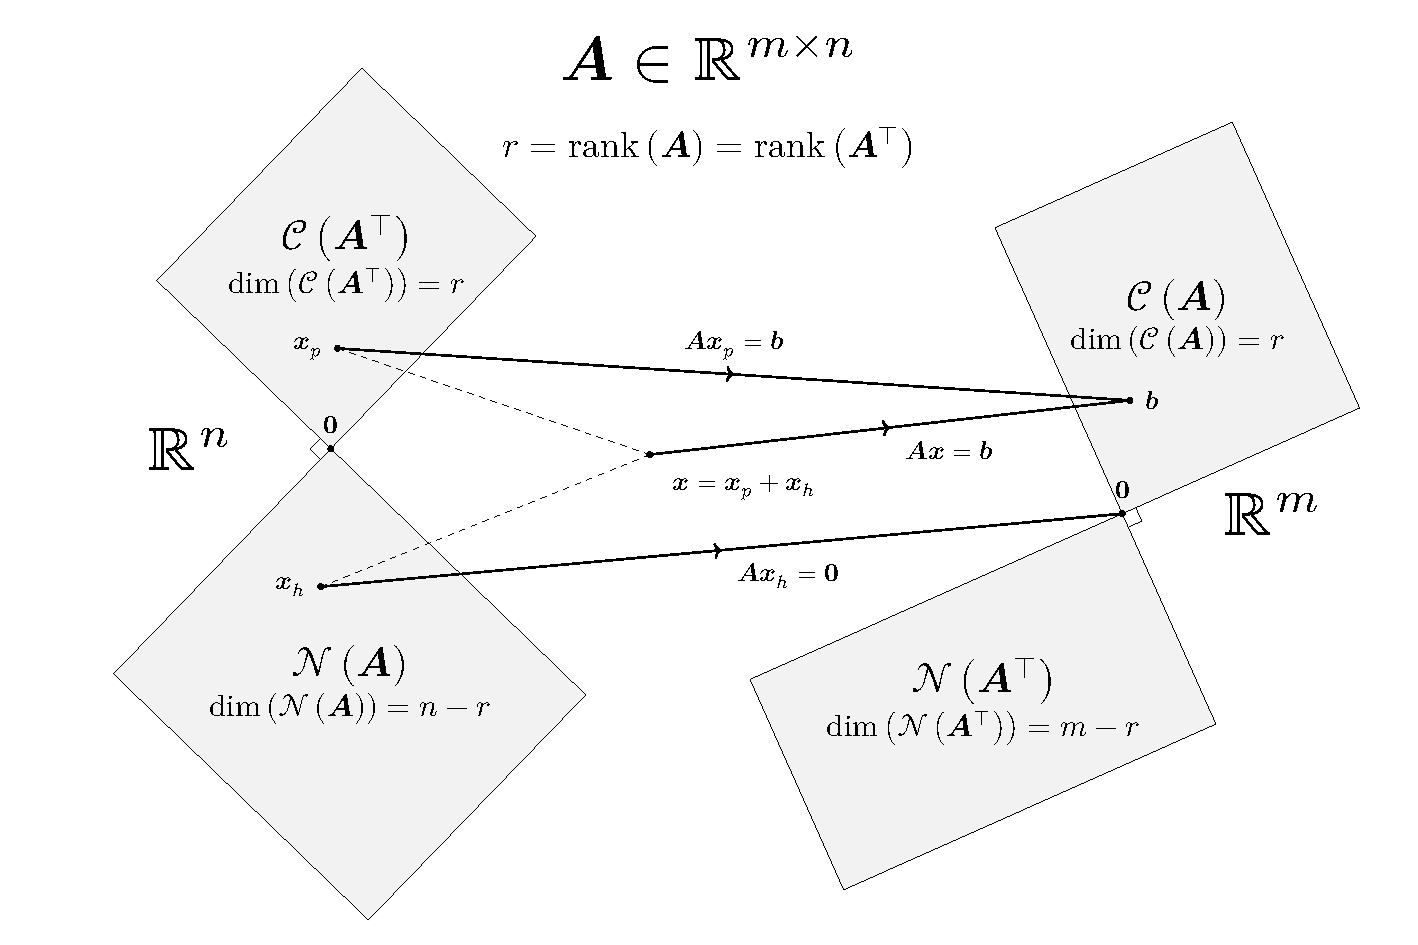
\includegraphics[height=10cm, keepaspectratio]{fundamental_subspaces.pdf}
		\caption{The Four Fundamental Subspaces of a Matrix.}
	\end{figure}
	\subsection{The Four Fundamental Subspaces of a Matrix}
	\begin{definition}
		If $\symbfit{A}\in\mathbb{R}^{m \times n}$ is an $m \times n$ matrix, then:
		\begin{enumerate}
			\item The subspace spanned by the \textit{column vectors} of $\symbfit{A}$, is the \textbf{column space} of $\symbfit{A}$, denoted $\columnspace{A}$.
			\item The subspace spanned by the \textit{row vectors} of $\symbfit{A}$, is the \textbf{row space} of $\symbfit{A}$, denoted $\rowspace{A}$.
			\item The subspace spanned by the \textit{solution space} of the equation $\symbfit{A}\symbfit{x}=\symbfup{0}$, is the \textbf{null space} of $\symbfit{A}$, denoted $\nullspace{A}$.
			\item The subspace spanned by the \textit{solution space} of the equation $\symbfit{A}^{\top}\symbfit{y}=\symbfup{0}$ (or $\symbfit{y}^{\top}\symbfit{A}=\symbfup{0}$), is the \textbf{left null space} of $\symbfit{A}$, denoted $\leftnullspace{A}$.
		\end{enumerate}  
	\end{definition}
	\subsection{The General Solution of a System of Equations}
	\begin{theorem}
		The \textbf{general solution} to a matrix equation $\symbfit{A}\symbfit{x}=\symbfit{b}$, can be given by adding the \underline{particular} and \underline{homogeneous} solutions, where the particular solution is the solution to $\symbfit{A}\symbfit{x}=\symbfit{b}$, or $\rowspace{A}$, and the homogeneous solution is the solution to $\symbfit{A}\symbfit{x}=\symbfup{0}$, or $\nullspace{A}$.
		\begin{equation*}
			\symbfit{x} = \symbfit{x}_p + \symbfit{x}_h
		\end{equation*}
	\end{theorem}
	\subsection{Row Equivalence}
	\begin{definition}
		Two matrices are \textbf{row equivalent} if each can be obtained from the other by elementary row operations. These matrices have the same \underline{row space} and \underline{null space}. 
	\end{definition}
	\subsection{Rank}
	\begin{definition}
		The \textbf{rank} of a matrix, denoted by $\rank{\left( \symbfit{A} \right)}$, is given by $\dim{\left( \columnspace{A} \right)}$.
	\end{definition}
	\begin{theorem}
		The column space and row space have the same dimension so that 
		\begin{equation*}
			\rank{\left( \symbfit{A} \right)}=\dim{\left( \columnspace{A} \right)}=\dim{\left( \rowspace{A} \right)}
		\end{equation*}
	\end{theorem}
	\subsection{Nullity}
	\begin{definition}
		The \textbf{nullity} of a matrix, denoted by $\vnull{\left( \symbfit{A} \right)}$, is given by $\dim{\left( \nullspace{A} \right)}$.
	\end{definition}
	\newpage
\section{Orthogonality}
	\begin{definition}
		Two vectors are \textbf{orthogonal} if the following holds.
		\begin{equation*}
			\symbfit{v}\cdot \symbfit{w}=0 \iff \symbfit{v}^{\top}\symbfit{w}=0
		\end{equation*}
	\end{definition}
	\begin{theorem}
		$\symbfup{0}$ is orthogonal to every vector in $V$.
	\end{theorem}
	\begin{theorem}
		$\symbfup{0}$ is the only vector in $V$, that is orthogonal to itself.
	\end{theorem}
	\begin{theorem}
		\begin{equation*}
			\norm{\symbfit{v}}^2=\symbfit{v}^{\top}\symbfit{v}
		\end{equation*}
	\end{theorem}
	\begin{theorem}
		\begin{equation*}
			\norm{\symbfit{v}}=\sqrt{\symbfit{v}^{\top}\symbfit{v}}
		\end{equation*}
	\end{theorem}
	\subsection{Orthogonal Subspaces}
	\begin{definition}
		Two subspaces $U$ and $W$ of a vector space $V$, are \textbf{orthogonal subspaces} iff every vector in $U$ is orthogonal to every vector in $W$.
		\begin{equation*}
			\forall \symbfit{u}\in U:\forall \symbfit{w}\in W:\symbfit{u}^{\top}\symbfit{w}=0
		\end{equation*}
	\end{definition}
	\subsection{Orthogonal Complements}
	\begin{definition}
		If $U$ is a subspace of $V$, then the \textbf{orthogonal complement} of $U$, denoted $U^{\perp}$, is the set of all vectors in $V$ that are orthogonal to every vector in $U$.
		\begin{equation*}
			U^{\perp} = \left\{ \forall \symbfit{u}\in U:\symbfit{v}\in V: \symbfit{v}^{\top}\symbfit{u}=0 \right\}
		\end{equation*}
	\end{definition}
	\begin{theorem}
		\begin{equation*}
			\left( U^{\perp} \right)^{\perp}=U
		\end{equation*}
	\end{theorem}
	\begin{theorem}
		\begin{equation*}
			\dim{U} + \dim{U^{\perp}} = \dim{V}
		\end{equation*}
	\end{theorem}
	\subsection{Vector Projections}
	\begin{figure}[H]
		\centering
		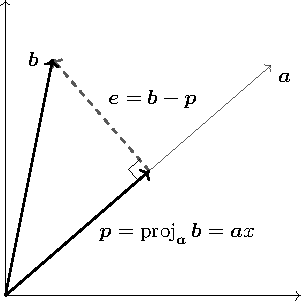
\includegraphics[height=5cm, keepaspectratio]{figures/vector_projection.pdf}
		\caption{Vector Projection of $\symbfit{b}$ onto $\symbfit{a}$.}
	\end{figure}
	\begin{definition}
		Let the \textbf{vector projection} of $\symbfit{b}$ onto $\symbfit{a}$, denoted as $\proj_{\symbfit{a}}\symbfit{b}$, be the \linebreak \underline{orthogonal projection} of $\symbfit{b}$ in the direction of $\symbfit{a}$, that minimises the error vector: $\symbfit{e}=\symbfit{b}-\symbfit{p}$.
	\end{definition}
	\begin{theorem}
	The projection of $\symbfit{b}$ onto $\symbfit{a}$ is given by
	\begin{equation*}
		\proj_{\symbfit{a}}\symbfit{b} = \symbfit{a} x = \symbfit{a} \left( \symbfit{a}^\top \symbfit{a} \right)^{-1}\symbfit{a}^\top \symbfit{b}
	\end{equation*}
	alternatively
	\begin{equation*}
		\proj_{\symbfit{a}}\symbfit{b} = \symbfit{a} x = \symbfit{a} \frac{\symbfit{a}^\top \symbfit{b}}{\symbfit{a}^\top \symbfit{a}} = \symbfit{a} \frac{\symbfit{a}\cdot\symbfit{b}}{\symbfit{a}\cdot\symbfit{a}}
	\end{equation*}
	\end{theorem}
	\begin{solution}[Proof]
		As $\symbfit{p}$ lies on line through $\symbfit{a}$, $\symbfit{p}=\symbfit{a}x$, so that $\symbfit{e}=\symbfit{b}-\symbfit{a}x$. As $\symbfit{e}$ is orthogonal to $\symbfit{a}$, we can construct the following relationship.
		\begin{align*}
			\symbfit{a}^\top \symbfit{e} &= 0 \\
			\symbfit{a}^\top \left( \symbfit{b} - \symbfit{a}x \right) &= 0 \\
			\symbfit{a}^\top \symbfit{b} - \symbfit{a}^\top \symbfit{a}x &= 0 \\
			\symbfit{a}^\top \symbfit{a}x &= \symbfit{a}^\top \symbfit{b} \\
			x &= \left( \symbfit{a}^\top \symbfit{a} \right)^{-1}\symbfit{a}^\top \symbfit{b} = \frac{\symbfit{a}^\top \symbfit{b}}{\symbfit{a}^\top \symbfit{a}}
		\end{align*}
	\end{solution}
	\subsection{Projection onto a Subspace}
	\begin{theorem}
		Let $W$ be a subspace of the vector space $V$ such that if $\symbfit{b}\in V$, then $\symbfit{p}=\proj_{W}\symbfit{b}$ is the \textbf{best approximation} of $\symbfit{b}$ on $W$, so that
		\begin{equation*}
			\norm{\symbfit{b}-\symbfit{p}}<\norm{\symbfit{b}-\symbfit{w}}
		\end{equation*}
		for all $\symbfit{w}\in W$, where $\symbfit{w}\neq \symbfit{p}$.
	\end{theorem}
	\begin{theorem}
		The projection of $\symbfit{b}$ onto the vector space $W$ is given by
		\begin{equation*}
			\proj_{W}\symbfit{b} = \symbfit{A}\symbfit{\hat{x}} = \symbfit{A}\left( \symbfit{A}^\top \symbfit{A} \right)^{-1}\symbfit{A}^\top \symbfit{b}
		\end{equation*}
	\end{theorem}
	\begin{solution}[Proof]
		As $\symbfit{p}\in W$, $\symbfit{p}$ can be represented as the linear combination of the basis vectors $\symbfit{a}_i$ that span $W$.
		\begin{align*}
			\symbfit{p} &= \hat{x}_1 \symbfit{a}_1 + \hat{x}_2 \symbfit{a}_2 + \dots + \hat{x}_n \symbfit{a}_n \\
			&= \mqty[
					\vertbar & \vertbar & & \vertbar \\ 
					\symbfit{a}_1 & \symbfit{a}_2 & \cdots & \symbfit{a}_n \\ 
					\vertbar & \vertbar & & \vertbar
				] 
				\mqty[
					\hat{x}_1 \\ 
					\hat{x}_2 \\ 
					\cdots \\ 
					\hat{x}_n
				] \\
			&= \symbfit{A}\symbfit{\hat{x}}
		\end{align*}
		Consider the error vector $\symbfit{e}=\symbfit{b}-\symbfit{p}$. As $\symbfit{e}$ is orthogonal to $W$, it will also be orthogonal to the vectors that span $W$. Therefore
		\begin{equation*}
			\left\{
				\begin{aligned}
					\symbfit{a}_1^\top\left( \symbfit{b}-\symbfit{A}\symbfit{\hat{x}} \right) &= 0 \\
					\symbfit{a}_2^\top\left( \symbfit{b}-\symbfit{A}\symbfit{\hat{x}} \right) &= 0 \\
					\vdotswithin{\symbfit{a}_3^\top}\phantom{\left( \symbfit{b}-\symbfit{A}\symbfit{\hat{x}} \right)} & \\
					\symbfit{a}_n^\top\left( \symbfit{b}-\symbfit{A}\symbfit{\hat{x}} \right) &= 0 
				\end{aligned}
			\right.
		\end{equation*}
		which gives the following equation
		\begin{equation*}
			\symbfit{A}^\top \left( \symbfit{b}-\symbfit{A}\symbfit{\hat{x}} \right) = \symbfup{0}
		\end{equation*}
		where we solve for $\symbfit{\hat{x}}$
		\begin{align*}
			\symbfit{A}^\top \symbfit{b}-\symbfit{A}^\top \symbfit{A}\symbfit{\hat{x}} &= \symbfup{0} \\
			\symbfit{A}^\top \symbfit{A}\symbfit{\hat{x}} &= \symbfit{A}^\top \symbfit{b} \\
			\symbfit{\hat{x}} &= \left( \symbfit{A}^\top \symbfit{A} \right)^{-1}\symbfit{A}^\top \symbfit{b}
		\end{align*}
	\end{solution}
	\subsection{Least Squares}
	\begin{theorem}
		Suppose $\symbfit{A}\symbfit{x}=\symbfit{b}$ is an \underline{inconsistent} linear system. The \textbf{least squares} solution of $\symbfit{A}\symbfit{x}=\symbfit{b}$ is given by the orthogonal projection $\proj_{\columnspace{A}}\symbfit{b}$.
	\end{theorem}
	\newpage
\section{Linear Maps}
	\subsection{Matrix Transformations}
	\begin{definition}
		A \textbf{matrix transformation} $T_{\symbfit{A}}:\mathbb{R}^n\rightarrow \mathbb{R}^m$ is a mapping of the form
		\begin{equation*}
			T_{\symbfit{A}}\left(\symbfit{x}\right) = \symbfit{A}\symbfit{x}
		\end{equation*}
		where $\symbfit{A}\in \mathbb{R}^{m \times n}$. As this transformation is linear, the following linearity properties hold.
		\begin{enumerate}
			\item $T\left(\symbfit{u}+\symbfit{v}\right)=T\left(\symbfit{u}\right) + T\left(\symbfit{v}\right)$
			\item $T\left(k\symbfit{u}\right)= kT\left(\symbfit{u}\right)$
		\end{enumerate}
	\end{definition}
	\subsection{General Linear Transformations}
	\begin{theorem}
		If $T: V \rightarrow W$ is a mapping between two vector spaces $V$ and $W$, then $T$ is the \textbf{linear transformation} from $V$ to $W$, and the following properties hold.
		\begin{enumerate}
			\item $T\left(\symbfit{u}+\symbfit{v}\right)=T\left(\symbfit{u}\right) + T\left(\symbfit{v}\right)$
			\item $T\left(k\symbfit{u}\right) kT\left(\symbfit{u}\right)$
		\end{enumerate}
	\end{theorem}
	\begin{theorem}
		When $V=W$, the linear map is called a \textbf{linear operator}.
	\end{theorem}
	\subsection{Subspaces of Linear Transformations}
	\begin{figure}[H]
		\centering
		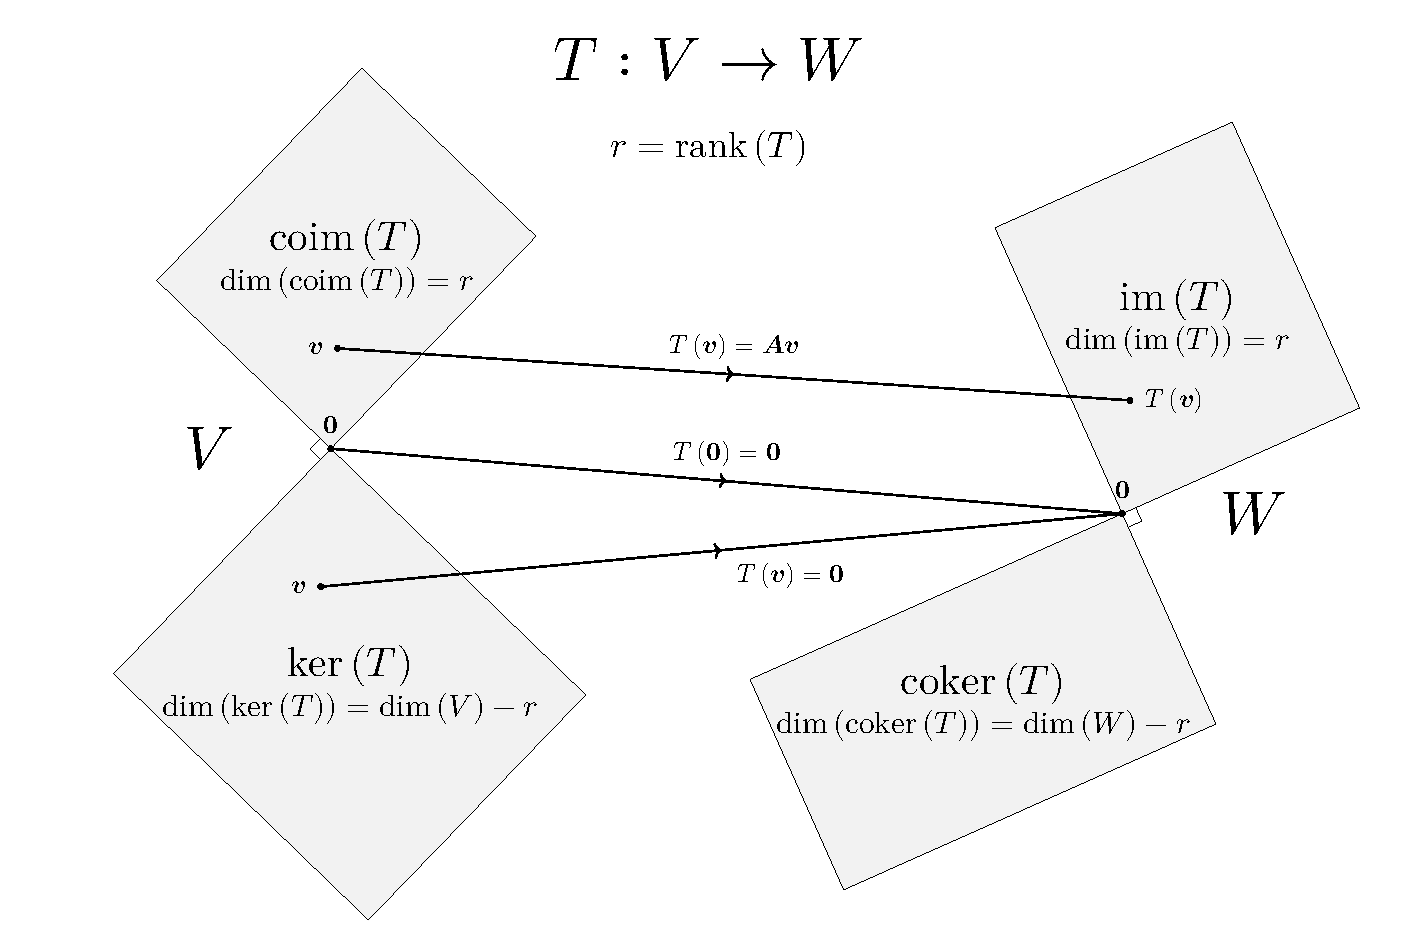
\includegraphics[height=10cm, keepaspectratio]{matrix_transformation}
		\caption{Subspaces of a Linear Transformation.}
	\end{figure}
	\begin{definition}
		If $T:V \rightarrow W$ is a linear transformation between two vector spaces $V$ and $W$, then:
		\begin{enumerate}
			\item The vector space $V$ is the \textbf{domain} of $T$.
			\item The vector space $W$ is the \textbf{codomain} of $T$.
			\item The \textbf{image} (or \textbf{range}) of $T$ is the set of vectors the linear transformation maps to.
			\begin{equation*}
				\vim{\left( T \right)} = T\left(V\right) = \left\{ T\left(\symbfit{v}\right) : \symbfit{v}\in V \right\} \subset W
			\end{equation*}
			\item The \textbf{kernel} of $T$ is the set of vectors that map to the zero vector.
			\begin{equation*}
				\vker{\left( T \right)} = \left\{ \symbfit{v}\in V : T\left(\symbfit{v}\right)=\symbfup{0} \right\}
			\end{equation*}
		\end{enumerate}
	\end{definition}
	\subsection{Constructing a Transformation Matrix}
	\begin{theorem}
		The standard matrix for a linear transformation is given by the formula:
		\begin{equation*}
			\symbfit{A} = \mqty[
				\vertbar & \vertbar & & \vertbar \\ 
				T\left(\symbfit{e}_1\right) & T\left(\symbfit{e}_2\right) & \cdots & T\left(\symbfit{e}_n\right) \\ 
				\vertbar & \vertbar & & \vertbar
			]
		\end{equation*}
		where
		\begin{equation*}
			\symbfit{e}_1 = \mqty[1 \\ 0 \\ 0 \\ \vdots \\ 0],\, \symbfit{e}_2 = \mqty[0 \\ 1 \\ 0 \\ \vdots \\ 0],\, \dots,\, \symbfit{e}_n = \mqty[0 \\ 0 \\ 0 \\ \vdots \\ 1]
		\end{equation*}
		are the \textbf{standard basis vectors} for $\mathbb{R}^n$.
	\end{theorem}
	\newpage
\section{Determinants}
	\subsection{Properties of Determinants}
	\begin{enumerate}
		\item $\det{\left( \mathbb{1} \right)}=1$.
		\item Exchanging two rows of a matrix reverses the sign of its determinant.
		\item Determinants are multilinear, so that 
		\begin{enumerate}[label=(\alph*)]
			\item $\mdet{a+a' & b+b' \\ c & d} = \mdet{a & b \\ c & d}+\mdet{a' & b' \\ c & d}$
			\item $\mdet{ta & tb \\ c & d}=t\mdet{a & b \\ c & d}$
		\end{enumerate}
		\item If $\symbfit{A}$ has two equal rows, then $\det{\left( \symbfit{A} \right)}=0$.
		\item Adding a scalar multiple of one row to another does not change the determinant of a matrix.
		\item If $\symbfit{A}$ has a row of zeros, then $\det{\left( \symbfit{A} \right)}=0$.
		\item If $\symbfit{A}$ is triangular, then $\det{\left( \symbfit{A} \right)}=\prod_{i=1}^{n} a_{ii}$.
		\item If $\symbfit{A}$ is singular, then $\det{\left( \symbfit{A} \right)}=0$.
		\item $\det{\left( \symbfit{A}\symbfit{B} \right)}=\det{\left( \symbfit{A} \right)}\det{\left( \symbfit{B} \right)}$.
		\item $\det{\left( \symbfit{A}^\top \right)}=\det{\left( \symbfit{A} \right)}$.
	\end{enumerate}
	\subsection{Matrix Minors}
	\begin{definition}
		The \textbf{minor} of $a_{ij}$ in $\symbfit{A}$, denoted $M_{ij}$, is the determinant of the submatrix formed by deleting the $i$th row and $j$th column of $\symbfit{A}$.
	\end{definition}
	\subsection{Matrix Cofactors}
	\begin{definition}
		The \textbf{cofactor} of $a_{ij}$ in $\symbfit{A}$ is defined as
		\begin{equation*}
			C_{ij} = \left( -1 \right)^{i+j} M_{ij}
		\end{equation*}
	\end{definition}
	\subsection{The Determinant of a Matrix}
	\begin{theorem}
		The determinant of an $n\times n$ matrix $\symbfit{A}$ is given by
		\begin{equation*}
			\det{\left( \symbfit{A} \right)} = \sum_{j=1}^n a_{ij}C_{ij} = \sum_{i=1}^n a_{ij}C_{ij}
		\end{equation*}
		where $a_{ij}$ is the entry in the $i$th row and $j$th column of $\symbfit{A}$.
	\end{theorem}
	\subsection{The Cofactor Matrix}
	\begin{definition}
		The \textbf{cofactor matrix} of an $n\times n$ matrix $\symbfit{A}$, denoted $\symbfit{C}$, is defined as the matrix of the cofactors of $\symbfit{A}$.
		\begin{equation*}
			\symbfit{C} = \mqty[
				C_{11} & C_{12} & \cdots & C_{1n} \\
				C_{21} & C_{22} & \cdots & C_{2n} \\
				\vdots & \vdots &        & \vdots \\
				C_{n1} & C_{n2} & \cdots & C_{nn}
				]
		\end{equation*}
	\end{definition}
	\subsection{The Adjugate of a Matrix}
	\begin{definition}
		The \textbf{adjugate} (or \textit{classical adjoint}) of a square matrix $\symbfit{A}$, denoted $\adj{\left( \symbfit{A} \right)}$, is the transpose its cofactor matrix.
		\begin{equation*}
			\adj{\left( \symbfit{A} \right)} = \symbfit{C}^\top
		\end{equation*}
	\end{definition}
	\subsection{The Inverse of a Matrix}
	\begin{theorem}
		The \textbf{inverse} of a nonsingular matrix $\symbfit{A}$ is given by 
		\begin{equation*}
			\symbfit{A}^{-1}=\frac{1}{\det{\symbfit{A}}} \adj{\left( \symbfit{A} \right)}
		\end{equation*}
	\end{theorem}
	\newpage
\section{Invariant Subspaces}
	\begin{definition}
		Consider the subspace $\mathcal{V}$ of the linear mapping $T:V\rightarrow V$ from a vector space $V$ to itself, then $\mathcal{V}$ is an \textbf{invariant subspace} of $T$ if
		\begin{equation*}
			T\left(\mathcal{V}\right)\subseteq \mathcal{V}
		\end{equation*}
	\end{definition}
	\begin{theorem}
		If $\mathcal{V}$ is an invariant subspace of a linear mapping $T: V \rightarrow V$ from a vector space $V$ to itself, then
		\begin{equation*}
			\forall \symbfit{v}\in \mathcal{V}\implies T\left(\symbfit{v}\right)\in \mathcal{V}
		\end{equation*}
	\end{theorem}
	\subsection{Trivial Invariant Subspaces}
	\begin{enumerate}
		\item $V$.
		\item $\left\{ \symbfup{0} \right\}$.
		\item $\vker{\left( T \right)}$.
		\item $\vim{\left( T \right)}$.
		\item Any linear combination of invariant subspaces.
	\end{enumerate}
	\subsection{Eigenspaces}
	\begin{definition}
		If an invariant subspace is one-dimensional, then the subspace is called an \textbf{eigenspace} of the linear transformation.
	\end{definition}
	\begin{theorem}
		If $\mathcal{V}$ is an eigenspace of the linear mapping $T: V \rightarrow V$, then
		\begin{equation*}
			\mathcal{V} = \left\{ \forall \symbfit{q}\in \mathcal{V}:\exists \lambda \in \mathbb{C}:T\left(\symbfit{q}\right)=\lambda \symbfit{q} \right\}
		\end{equation*}
		where $\lambda$ is the \textbf{eigenvalue} associated with the \textbf{eigenvector} $\symbfit{q}$.
	\end{theorem}
	\subsection{The Eigenvalue Problem}
	\begin{theorem}
		The eigenvalues $\lambda$ of an invertible square matrix $\symbfit{A}$, are the solutions to 
		\begin{equation*}
			\det{\left( \symbfit{A} - \lambda\mathbb{1} \right)}=\symbfup{0}
		\end{equation*} 
	\end{theorem}
	\begin{theorem}
		The eigenvectors associated with each eigenvalue, of an invertible square matrix $\symbfit{A}$, are the solutions to
		\begin{equation*}
			\left( \symbfit{A} - \lambda \mathbb{1} \right) \symbfit{q}=\symbfup{0}
		\end{equation*}
	\end{theorem}
	\begin{solution}[Proof]
	The eigenvalues and associated eigenvectors of a square matrix $\symbfit{A}$, are the solutions to $\symbfit{A}\symbfit{q}=\lambda \symbfit{q}$.
	\begin{align*}
		\symbfit{A}\symbfit{q}&=\lambda \symbfit{q} \\
		\symbfit{A}\symbfit{q} - \lambda \symbfit{q}&=\symbfup{0} \\
		\left( \symbfit{A} - \lambda \mathbb{1} \right) \symbfit{q}&=\symbfup{0}
	\end{align*}
	The linear system $\left( \symbfit{A} - \lambda\mathbb{1} \right) \symbfit{q}=\symbfup{0}$ has a nontrivial solution iff $\symbfit{A} - \lambda \mathbb{1}$ is singular.
	\end{solution}
	\subsection{Properties of Eigenvalues}
	\begin{theorem}
		\begin{equation*}
			\tr{\left( \symbfit{A} \right)} = \sum_{i=1}^n \lambda_i
		\end{equation*}
	\end{theorem}
	\begin{theorem}
		\begin{equation*}
			\det{\left( \symbfit{A} \right)} = \prod_{i=1}^n \lambda_i
		\end{equation*}
	\end{theorem}
	\newpage
\section{Eigen Decomposition}
	\subsection{Similarity Transformations}
	\begin{definition}
		A \textbf{similarity transformation} is a linear mapping of the form
		\begin{equation*}
			\symbfit{A}\rightarrow \symbfit{Q}^{-1}\symbfit{A}\symbfit{Q}
		\end{equation*}
		in which the matrices $\symbfit{A}$ and $\symbfit{Q}$ are $n \times n$ invertible matrices. Here we say, ``$\symbfit{A}$ is similar to $\symbfit{Q}^{-1}\symbfit{A}\symbfit{Q}$''.
	\end{definition}
	\subsection{Matrix Diagonalisation}
	\begin{definition}
		The matrix $\symbfit{A}$ is a \textbf{diagonalisable} matrix if it is similar to a diagonal matrix. That is, there exists an invertible matrix $\symbfit{Q}$, and diagonal matrix $\symbfit{\Lambda}$, such that
		\begin{equation*}
			\symbfit{\Lambda}=\symbfit{Q}^{-1}\symbfit{A}\symbfit{Q}
		\end{equation*}
	\end{definition}
	\begin{theorem}
		Let $\symbfit{A}$ be an $n \times n$ matrix with $n$ linearly independent eigenvectors, then $\symbfit{A}$ is diagonalisable if $\symbfit{\Lambda}=\diag{\left( \lambda_1,\: \lambda_2,\: \dots,\: \lambda_n \right)}$ and $\symbfit{Q}$ is a matrix composed of the eigenvectors of $\symbfit{A}$. Explicitly,
		\begin{equation*}
			\symbfit{\Lambda} = 
			\mqty[
				\lambda_1 & & & \\
				& \lambda_2 & & \\
				& & \ddots & \\
				& & & \lambda_n
				]\quad
				\text{and}\quad
			\symbfit{Q} = \mqty[
				\vertbar & \vertbar & & \vertbar \\ 
				\symbfit{q}_1 & \symbfit{q}_2 & \cdots & \symbfit{q}_n \\ 
				\vertbar & \vertbar & & \vertbar
			]
		\end{equation*}
		where $\symbfit{q}_1,\: \symbfit{q}_2,\: \dots,\: \symbfit{q}_n$ are the eigenvectors of $\symbfit{A}$.
	\end{theorem}
	\begin{solution}[Proof]
		Let $\symbfit{q}_1,\: \symbfit{q}_2,\: \dots,\: \symbfit{q}_n,$ be linearly independent eigenvectors of $\symbfit{A}$, and $\lambda_1,\: \lambda_2,\: \dots,\: \lambda_n$, the associated eigenvalues. By definition of an eigenspace, we have
		\begin{equation*}
			\left\{
			\setlength\arraycolsep{0pt}
			\begin{array}{ r >{{}}c<{{}} l }
				\symbfit{A}\symbfit{q}_1 &=& \lambda_1 \symbfit{q}_1 \\
				\symbfit{A}\symbfit{q}_2 &=& \lambda_2 \symbfit{q}_2 \\
				\vdotswithin{\symbfit{q}_3} & & \vdotswithin{\lambda_3}\vdotswithin{\symbfit{q}_3} \\
				\symbfit{A}\symbfit{q}_n &=& \lambda_n \symbfit{q}_n
			\end{array}
			\right.
		\end{equation*}
		which we can rewrite as
		\begin{align}
			\symbfit{A}\symbfit{Q} &= \symbfit{Q}\symbfit{\Lambda} \label{equation:eigenspace_matrix} \\
			\symbfit{\Lambda}&=\symbfit{Q}^{-1}\symbfit{A}\symbfit{Q} \nonumber 
		\end{align}
		by rearranging \hyperref[equation:eigenspace_matrix]{Equation \ref{equation:eigenspace_matrix}}, we have $\symbfit{A}$ in terms of its eigenvalues and eigenvectors.
		\begin{equation*}
			\symbfit{A} = \symbfit{Q}\symbfit{\Lambda} \symbfit{Q}^{-1}
		\end{equation*}
	\end{solution}
	\subsection{Powers of a Matrix}
	\begin{theorem}
		Let $\symbfit{A}$ be a diagonalisable matrix, then for all $k \in \mathbb{N}_0$
		\begin{equation*}
			\symbfit{A}^k = \symbfit{Q} \symbfit{\Lambda}^k \symbfit{Q}^{-1}
		\end{equation*}
	\end{theorem}
	\begin{solutionF}[Proof]
		\begin{align*}
			\symbfit{A}^k &= \left( \symbfit{Q} \symbfit{\Lambda} \symbfit{Q}^{-1} \right)^k \\
			&= \underbrace{\left( \symbfit{Q} \symbfit{\Lambda} \symbfit{Q}^{-1} \right)\left( \symbfit{Q} \symbfit{\Lambda} \symbfit{Q}^{-1} \right)\cdots\left( \symbfit{Q} \symbfit{\Lambda} \symbfit{Q}^{-1} \right)}_{\text{$k$ times}} \\
			&= \underbrace{\symbfit{Q} \symbfit{\Lambda} \symbfit{Q}^{-1} \symbfit{Q} \symbfit{\Lambda} \symbfit{Q}^{-1} \cdots \symbfit{Q} \symbfit{\Lambda} \symbfit{Q}^{-1} }_{\text{$k$ times}} \\
			&= \underbrace{\symbfit{Q} \symbfit{\Lambda} \cancel{\symbfit{Q}^{-1} \symbfit{Q}} \symbfit{\Lambda} \cancel{\symbfit{Q}^{-1} \cdots \symbfit{Q}} \symbfit{\Lambda} \symbfit{Q}^{-1} }_{\text{$k$ times}} \\
			&= \symbfit{Q} \underbrace{ \symbfit{\Lambda} \symbfit{\Lambda} \cdots \symbfit{\Lambda} }_{\text{$k$ times}}\symbfit{Q}^{-1} \\
			&= \symbfit{Q} \symbfit{\Lambda}^k\symbfit{Q}^{-1}
		\end{align*}
	\end{solutionF}
	\begin{theorem}
		The eigenvalues of $\symbfit{A}^k$, $\forall k \in \mathbb{N}$ are $\lambda_1^k,\: \lambda_2^k,\: \dots,\: \lambda_n^k$.
	\end{theorem}
	\begin{theorem}
		The eigenvectors of $\symbfit{A}$ are equal to the eigenvectors of $\symbfit{A}^k$.
	\end{theorem}
	\newpage
\section{System of Differential Equations}
	\subsection{First-Order Differential Equations}
	\begin{definition}
		A \textbf{first-order differential equation} is a differential equation where the highest derivative is of order one. 
		\begin{equation*}
			x' = a x
		\end{equation*}
	\end{definition}
	\begin{theorem}
		The general solution to a first-order linear differential equation is of the form
		\begin{equation*}
			x(t) = c_1 \e^{a t}
		\end{equation*}
		where $c_1$ is an arbitrary constant.
	\end{theorem}
	\subsection{First-Order System of Differential Equations}
	\begin{definition}
		A \textbf{first-order system of differential equations} is of the form
		\begin{equation*}
			\left\{
			\setlength\arraycolsep{0pt}
			\begin{array}{ c >{{}}c<{{}} c >{{}}c<{{}} c >{{}}c<{{}} c >{{}}c<{{}} c  }
			x'_1               &=& a_{11}x_1                         &+& a_{12}x_2                         &+& \cdots &+& a_{1n}x_n \\
			x'_2               &=& a_{21}x_1                         &+& a_{22}x_2                         &+& \cdots &+& a_{2n}x_n \\
			\vdotswithin{x'_3} & & \vdotswithin{a_{31}}\phantom{x_1} & & \vdotswithin{a_{32}}\phantom{x_2} & &        & & \vdotswithin{a_{3n}}\phantom{x_n} \\ 
			x'_n               &=& a_{n1}x_1                         &+& a_{n2}x_2                         &+& \cdots &+& a_{nn}x_n 
			\end{array}
			\right.
		\end{equation*}
		where $x_1=x_1(t),\: x_2=x_2(t),\: \dots,\: x_n=x_n(t)$ are the functions to be determined. In matrix form, the system can be written as
		\begin{align*}
			\dv{t}\mqty[x_1 \\ x_2 \\ \vdots \\ x_n] &= \mqty[
				a_{11} & a_{12} & \cdots & a_{1n} \\
				a_{21} & a_{22} & \cdots & a_{2n} \\
				\vdots & \vdots &        & \vdots \\
				a_{n1} & a_{n2} & \cdots & a_{nn}
			] \mqty[x_1 \\ x_2 \\ \vdots \\ x_n] \\
			\symbfit{x}' &= \symbfit{A} \symbfit{x}
		\end{align*}
	\end{definition}
	\subsection{Solution using Diagonalisation}
	\begin{theorem}
		The first-order system of differential equations $\symbfit{x}' = \symbfit{A} \symbfit{x}$ can be solved using the following substitution
		\begin{equation*}
			\symbfit{x}=\symbfit{Q}\symbfit{u}
		\end{equation*}
		where $\symbfit{u}$ is a vector to be determined, and $\symbfit{Q}$ is the matrix that diagonalises $\symbfit{A}$. $\symbfit{u}$ is determined by solving
		\begin{equation*}
			\symbfit{u}' = \symbfit{\Lambda} \symbfit{u}
		\end{equation*}
		where $\symbfit{\Lambda}$ is the diagonal similarity transformation of $\symbfit{A}$. This substitution uncouples the system of differential equations so that each equation can be solved as a first-order differential equation.
	\end{theorem}
	\begin{solutionF}[Proof]
		\begingroup 
		\allowdisplaybreaks
		\begin{align*}
			\symbfit{x}' &= \symbfit{A} \symbfit{x} \\
			\left( \symbfit{Q}\symbfit{u} \right)' &= \left( \symbfit{Q}\symbfit{\Lambda} \symbfit{Q}^{-1} \right)\left( \symbfit{Q}\symbfit{u} \right) \\
			\symbfit{Q}\symbfit{u}' &= \symbfit{Q}\symbfit{\Lambda} \symbfit{Q}^{-1} \symbfit{Q}\symbfit{u} \\
			\cancel{\symbfit{Q}}\symbfit{u}' &= \cancel{\symbfit{Q}}\symbfit{\Lambda} \cancel{\symbfit{Q}^{-1} \symbfit{Q}}\symbfit{u} \\
			\symbfit{u}' &= \symbfit{\Lambda} \symbfit{u}
		\end{align*}
		\endgroup
	\end{solutionF}
	\begin{theorem}
		If $\symbfit{A}$ is a diagonalisable matrix, then the general solution of $\symbfit{x}' = \symbfit{A} \symbfit{x}$ can be expressed as
		\begin{equation*}
			\symbfit{x}(t) = c_1 \e^{\lambda_1 t} \symbfit{q}_1 + c_2 \e^{\lambda_2 t} \symbfit{q}_2 + \cdots + c_n \e^{\lambda_n t} \symbfit{q}_n
		\end{equation*}
	\end{theorem}
	\subsection{Principle of Superposition}
	\begin{theorem}
		If $x_1$ and $x_2$ are two solutions to a linear differential equation, then
		\begin{equation*}
			x = c_1 x_1 + c_2 x_2
		\end{equation*}
		is also a solution to the differential equation.
	\end{theorem}
	\subsection{Higher-Order Differential Equations}
	\begin{theorem}
		A \textbf{higher-order linear differential equation} can be solved by first converting it to a first-order linear system. Consider the $n$th-order differential equation
		\begin{equation*}
			x^{\left( n \right)} + a_1 x^{\left( n-1 \right)} + \cdots + a_{n-1} x' + a_n x = 0
		\end{equation*}
		We then define
		\begin{align*}
			x_1 &= x \\
			x_2 &= x' \\
			&\vdotswithin{=} \\
			x_n &= x^{\left( n-1 \right)}
		\end{align*}
		Let $\symbfit{x}=\mqty[x_1 & x_2 & \cdots & x_n]^\top$. Then the first-order linear system of differential equations can be written as
		\begin{equation*}
			\dv{t}\mqty[
				x_1 \\
				x_2 \\
				\vdotswithin{x_3} \\
				x_n	
			] = \mqty[
				0 & 1 & 0 & \cdots & 0 \\
				0 & 0 & 1 & \cdots & 0 \\
				\vdots & \vdots & \vdots & \ddots & \vdots \\
				0 & 0 & 0 & \cdots & 1 \\
				-a_n & -a_{n-1} & -a_{n-2} & \cdots & -a_1
			] \mqty[
				x_1 \\
				x_2 \\
				\vdotswithin{x_3} \\
				x_n	
			]
		\end{equation*}
	\end{theorem}
\newpage

\listoffigures 

\newpage

\nocite{*}

\bibliographystyle{plainurl}
\bibliography{MXB106_Lecture_Notes.bib}

\end{document}